\newcommand{\BLEU}{\textsc{Bleu}}

\hypertarget{the-im2latex-problem}{%
\section{\texorpdfstring{The \texttt{im2latex}
problem}{The im2latex problem}}\label{the-im2latex-problem}}

\begin{itemize}
\tightlist
\item
  Math Image to Math Code
\end{itemize}

\begin{figure}
\centering
\includegraphics{assets/attn_model.png}
\caption{Attention Model: Prediction over time-steps. Credit: Bender}
\end{figure}

\hypertarget{accomplishments}{%
\section{Accomplishments}\label{accomplishments}}

\begin{itemize}
\item
  Synthesized Dataset from Scratch
\item
  500,000 text examples!
\item
  170,000 original example images (700MB)

  \begin{itemize}
  \tightlist
  \item
    Deng used 100k and Singh 140k
  \end{itemize}
\item
  2 Models Trained and Ready for Inference! (800MB)
\end{itemize}

\hypertarget{state-of-the-art-in-im2latex}{%
\section{\texorpdfstring{State of the Art in
\texttt{im2latex}}{State of the Art in im2latex}}\label{state-of-the-art-in-im2latex}}

\begin{longtable}[]{@{}lll@{}}
\toprule
Researchers & BLEU Score (\%) & Training Time\tabularnewline
\midrule
\endhead
Deng et al 2017 & 87.73 & 20 hours\tabularnewline
Genthial 2017 & 88.00 & -\tabularnewline
Wang, Sun \& Wang 2018 & 88.25 & -\tabularnewline
Singh 2018 & 89.00 & 60 hours\tabularnewline
\textbf{Taradachuk \& Vente} & 88.48 & 75 hours\tabularnewline
Wang \& Liu 2019 & 90.28 & 75 hours\tabularnewline
\bottomrule
\end{longtable}

\hypertarget{our-data-processing-pipeline}{%
\section{Our Data Processing
Pipeline}\label{our-data-processing-pipeline}}

\begin{figure}
\centering
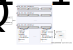
\includegraphics{assets/harvest.pdf}
\caption{Preprocessing Steps}
\end{figure}

\hypertarget{interpreting-bleu-score}{%
\section{Interpreting BLEU Score}\label{interpreting-bleu-score}}

\begin{itemize}
\tightlist
\item
  Let \(p_i\) be geometric mean of \(n\)-gram precisions
\end{itemize}

\hypertarget{brevity-pentalty}{%
\subsection{Brevity Pentalty}\label{brevity-pentalty}}

\begin{equation}
 \text{BP} = \begin{cases}1 &\text{ if } c>r \\
  e^{1-r/c} &\text{ otherwise }\end{cases}.
\end{equation}

\hypertarget{calculation}{%
\subsection{Calculation}\label{calculation}}

\begin{equation}
  \text{\textsc{Bleu}} = \text{BP} \exp\left( \sum_{i=1}^n w_i \log p_i \right)
\end{equation}

Note\footnote{The following are simplified contrived examples, using 4-gram BLEU
score. For a more complete picture see Papineni, Roukos, Ward, et al.}

\hypertarget{example-1}{%
\section{Example 1}\label{example-1}}

\begin{Shaded}
\begin{Highlighting}[]
\NormalTok{reference }\OperatorTok{=}\NormalTok{ [}
\NormalTok{  [}\StringTok{\textquotesingle{}the\textquotesingle{}}\NormalTok{, }\StringTok{\textquotesingle{}quick\textquotesingle{}}\NormalTok{, }\StringTok{\textquotesingle{}brown\textquotesingle{}}\NormalTok{, }\StringTok{\textquotesingle{}fox\textquotesingle{}}\NormalTok{,}
  \StringTok{\textquotesingle{}jumped\textquotesingle{}}\NormalTok{, }\StringTok{\textquotesingle{}over\textquotesingle{}}\NormalTok{, }\StringTok{\textquotesingle{}the\textquotesingle{}}\NormalTok{, }\StringTok{\textquotesingle{}lazy\textquotesingle{}}\NormalTok{, }\StringTok{\textquotesingle{}dog\textquotesingle{}}\NormalTok{]}
\NormalTok{]}
\NormalTok{candidate }\OperatorTok{=}
\NormalTok{  [}\StringTok{\textquotesingle{}the\textquotesingle{}}\NormalTok{, }\StringTok{\textquotesingle{}quick\textquotesingle{}}\NormalTok{, }\StringTok{\textquotesingle{}brown\textquotesingle{}}\NormalTok{, }\StringTok{\textquotesingle{}fox\textquotesingle{}}\NormalTok{,}
  \StringTok{\textquotesingle{}jumped\textquotesingle{}}\NormalTok{, }\StringTok{\textquotesingle{}over\textquotesingle{}}\NormalTok{, }\StringTok{\textquotesingle{}the\textquotesingle{}}\NormalTok{, }\StringTok{\textquotesingle{}lazy\textquotesingle{}}\NormalTok{, }\StringTok{\textquotesingle{}dog\textquotesingle{}}\NormalTok{]}
\BuiltInTok{print}\NormalTok{(sentence\_bleu(reference, candidate))}
\end{Highlighting}
\end{Shaded}

\begin{itemize}
\tightlist
\item
  1.0
\end{itemize}

\hypertarget{example-2}{%
\section{Example 2}\label{example-2}}

\begin{Shaded}
\begin{Highlighting}[]
\NormalTok{reference }\OperatorTok{=}\NormalTok{ [}
\NormalTok{  [}\StringTok{\textquotesingle{}the\textquotesingle{}}\NormalTok{, }\StringTok{\textquotesingle{}quick\textquotesingle{}}\NormalTok{, }\StringTok{\textquotesingle{}brown\textquotesingle{}}\NormalTok{, }\StringTok{\textquotesingle{}fox\textquotesingle{}}\NormalTok{,}
  \StringTok{\textquotesingle{}jumped\textquotesingle{}}\NormalTok{, }\StringTok{\textquotesingle{}over\textquotesingle{}}\NormalTok{, }\StringTok{\textquotesingle{}the\textquotesingle{}}\NormalTok{, }\StringTok{\textquotesingle{}lazy\textquotesingle{}}\NormalTok{, }\StringTok{\textquotesingle{}dog\textquotesingle{}}\NormalTok{]}
\NormalTok{]}
\NormalTok{candidate }\OperatorTok{=}
\NormalTok{  [}\StringTok{\textquotesingle{}the\textquotesingle{}}\NormalTok{, }\StringTok{\textquotesingle{}FAST\textquotesingle{}}\NormalTok{, }\StringTok{\textquotesingle{}brown\textquotesingle{}}\NormalTok{, }\StringTok{\textquotesingle{}fox\textquotesingle{}}\NormalTok{,}
  \StringTok{\textquotesingle{}jumped\textquotesingle{}}\NormalTok{, }\StringTok{\textquotesingle{}over\textquotesingle{}}\NormalTok{, }\StringTok{\textquotesingle{}the\textquotesingle{}}\NormalTok{, }\StringTok{\textquotesingle{}lazy\textquotesingle{}}\NormalTok{, }\StringTok{\textquotesingle{}dog\textquotesingle{}}\NormalTok{]}
\BuiltInTok{print}\NormalTok{(sentence\_bleu(reference, candidate))}
\end{Highlighting}
\end{Shaded}

\begin{itemize}
\item
  1 wrong token at length 9
\item
  0.7506\ldots{}
\end{itemize}

\hypertarget{notes-and-take-aways}{%
\section{Notes and Take-Aways}\label{notes-and-take-aways}}

\begin{itemize}
\item
  real data will account for synonyms
\item
  steep penalty for any bad tokens on short sequences
\item
  to (really) simplify missing words and extra words ``count as
  incorrect''
\end{itemize}

\hypertarget{distribution-of-input-length}{%
\section{Distribution of Input
Length}\label{distribution-of-input-length}}

\includegraphics{assets/histogram.pdf}

\hypertarget{distribution-of-scores}{%
\section{Distribution of Scores}\label{distribution-of-scores}}

\includegraphics{assets/scorehistogram.pdf}

\hypertarget{distribution-of-scores-1}{%
\section{Distribution of Scores}\label{distribution-of-scores-1}}

\includegraphics{assets/scorebyfrac.pdf}

\hypertarget{distribution-of-scores-2}{%
\section{Distribution of Scores}\label{distribution-of-scores-2}}

\includegraphics{assets/scorebylen.pdf}

\hypertarget{distribution-of-scores-3}{%
\section{Distribution of Scores}\label{distribution-of-scores-3}}

\includegraphics{assets/scorebylenstacked.pdf}

\hypertarget{demo-time}{%
\section{Demo Time}\label{demo-time}}

\begin{itemize}
\tightlist
\item
  Sample Images from the class!
\end{itemize}

\hypertarget{special-thanks}{%
\section{Special Thanks}\label{special-thanks}}

\begin{itemize}
\item
  Brian Newbold (archivist)
\item
  Sumeet S. Singh (works at Turnitin (Gradescope) now )
\end{itemize}

\hypertarget{improvement-points}{%
\section{Improvement Points}\label{improvement-points}}

\begin{itemize}
\item
  used command line for processing

  \begin{itemize}
  \item
    allowed rapid iteration, \emph{but}
  \item
    should've been python scripts
  \end{itemize}
\item
  Tensorflow 2.0 differences made translation prohibitive

  \begin{itemize}
  \tightlist
  \item
    Kept to the last stable release on the 1.0 branch
  \end{itemize}
\end{itemize}

\hypertarget{questions}{%
\section{Questions?}\label{questions}}

\begin{itemize}
\item
  Ask Us about\ldots{}

  \begin{itemize}
  \item
    ANN structure,
  \item
    Virtual Machine; or
  \item
    The models better than ours.
  \end{itemize}
\end{itemize}
